%%This is a very basic article template.
%%There is just one section and two subsections.
\documentclass[a4paper,11pt]{article}
\usepackage[pdfborder= 0 0 0 1]{hyperref}
\usepackage{graphicx}
\usepackage{appendix}
\usepackage{tabularx}
\usepackage[usenames,dvipsnames,svgnames,table]{xcolor}
\usepackage[spanish]{babel}
\usepackage{listings}
\usepackage{amsmath}
\definecolor{light-gray}{gray}{0.9}
\definecolor{dark-gray}{gray}{0.375}
\lstset{ %
   language=Matlab,                % choose the language of the code
   basicstyle=\scriptsize,       % the size of the fonts that are used for the
   numbers=left,                   % where to put the line-numbers
   numberstyle=\tiny\color{dark-gray},      % the size of the fonts that are used for the
   stepnumber=1,                   % the step between two line-numbers. If it is
   numbersep=5pt,                  % how far the line-numbers are from the code
   backgroundcolor=\color{light-gray},  % choose the background color. You must add
   showspaces=false,               % show spaces adding particular underscores
   showstringspaces=false,         % underline spaces within strings
   showtabs=false,                 % show tabs within strings adding particular
   flexiblecolumns=false,
   frame=single,                   % adds a frame around the code
   captionpos=b,                   % sets the caption-position to bottom
   breaklines=true,                % sets automatic line breaking
   breakatwhitespace=false,        % sets if automatic breaks should only happen at
   escapeinside={\%*}{*)}
}
%%\usepackage{draftwatermark}
%%\SetWatermarkLightness{0.9}
%%\SetWatermarkScale{5}
\begin{document}

\selectlanguage{spanish}

\title{\textbf{{\LARGE TIP entrega 1 \\ curso 2012/2013}}}
\author{Carlos Gil Soriano\\UAM-HPCN\\
\hypersetup{
  colorlinks   =  true,
  urlcolor     =  blue
  pdftitle     = {TIP entrega 1 \\ curso 2012/2013},
  pdfauthor    = {Carlos Gil Soriano},
  pdfsubject   = {TIP exercise 1, course 2012/2013},
  pdfkeywords  = {Euler, SDF, Brownian, Newton-Rhapson, quadrature, Normal pdf}
}
\href{mailto:gilsoriano@gmail.com}{\textbf{\textit{gilsoriano@gmail.com}}}}
\date{\today}
\maketitle
\thispagestyle{empty}
\begin{figure}[htb]
   \begin{center}
      
\includegraphics[scale=1,
      keepaspectratio]{../../../../../figures/logo/logo-uam.jpg}
   \end{center}
\end{figure}

\begin{abstract}

   En esta primera entrega de ejercicios se tratan tres problemas que se centran
   en:
   \begin{itemize}
      \item Comparaci\'on del c\'alculo de momentos de orden n mediante
         \textit{cuadraturas} con su correspondiente mediante simulaci\'on por
         \textit{Montecarlo}.
      \item Propiedades del \textit{Browniano aritm\'etico}.
      \item Aplicaciones del \textit{Browniano geom\'etrico}.
   \end{itemize}

\end{abstract}

\vspace{2cm}
\begin{center}
\begin{tabular}{|p{2.5cm}|p{3.5cm}|p{3.5cm}|}
\hline
\multicolumn{3}{|c|}{\textbf{Historial}}\\
\hline
\hline
\textbf{Versi\'on} & \textbf{Estado} & \textbf{Fecha}\\
\hline
0.1 & Problema 1 resuelto & 18 de febrero de 2013\\
\hline
0.2 & Problema 2 resuelto & 19 de febrero de 2013\\
\hline
1.0 & Problema 3 resuelto & 21 de febrero de 2013\\
\hline
\end{tabular}
\end{center}

\newpage
\mbox{}
\thispagestyle{empty}
\pagebreak

\pagenumbering{roman}
\setcounter{page}{1}
\pagebreak

\setcounter{tocdepth}{3}
\tableofcontents
\pagebreak
\listoftables
\listoffigures
\lstlistoflistings
\pagebreak

\pagenumbering{arabic}
\setcounter{page}{1}

\pagebreak
\section{C\'alculo de momentos centrales}

Se define un momento central de orden n como:\\
\begin{equation*}
   \mu_n = E [(X- E[X])^n] = \int_{-\infty}^\infty (x - \mu)^n pdf(x)dx
\end{equation*}

Para realizar la cuadratura debemos identificar la funci\'on $g(x)$ a
integrar:\\
\begin{equation*}
   I = \int_{-\infty}^\infty g(x)dx
\end{equation*}

En nuestro caso se trata de:\\
\begin{equation*}
   g(x) = (x - \mu)^n pdf(x)
\end{equation*}

g(x) se ha definido en Matlab en la funci\'on
\hyperref[quadfunc]{\textit{quadfunction.m}}. La integraci\'on por cuadratura de
Lobatto (cuadratura gaussiana con peso constante de 1) se realiza en Matlab por
medio del comando \textit{quadl}. El c\'odigo del c\'alculo de
$\mathcal{N}(\mu, \sigma)$ se encuentra en
\hyperref[centralMomentQuad]{\textit{centralMomentGaussian.m}}.
%\begin{center}
%\begin{tabularx}{\textwidth}{|X|}
%\hline
%It is recommended to take a look to the I2C standard before continue reading.\\
%\hline
%\end{tabularx}
%\end{center}

\subsection{Salida del programa y evaluaci\'on}

\begin{lstlisting}
>> mu = 0; sigma = 1;
   N = 8;
   for n = 1:N;
   moment(n) = centralMomentGaussian(mu,sigma,n);
   end
   moment

moment =
4.0305e-22

moment =
1.0000

moment =
4.0305e-20

moment =
3.0000

moment =
4.0305e-18

moment =
15.0000

moment =
-4.1039e-17

moment =
105.0000

moment =
0.000   1.000   0.000   3.000   0.000   15.000   -0.000   105.000
\end{lstlisting}

Se observa que el primer y segundo momento ofrecen los valores esperados de cero y
varianza, respectivamente. Adem\'as, dada la simetr\'ia de la funci\'on a
integrar, g(x), y la simetr\'ia del dominio de integraci\'on, se comprueba que
los momentos de orden impar se anulan.

\subsection{Comparaci\'on con simulaci\'on por Montecarlo}
La simulaci\'on por el m\'etodo de Montecarlo en \textit{demoCentralMomentGaussianMC}
ofrece unos resultados similares:
\begin{itemize}
   \item El histograma de los momentos de orden impar se concentra sobre cero.
   \item El histograma de momentos de orden 2, se concentra sobre la varianza.
\end{itemize}

\pagebreak
\section{Propiedades browniano aritm\'etico}
El \textbf{browniano aritm\'etico}, tambi\'en llamado proceso de Wiener con deriva $\mu$ y
varianza $\sigma^2$, es de la forma:

\begin{equation*}
   \tag{\textbf{ABM}}
   dS_t = \mu dt + \sigma dW_t
\end{equation*}

Se muestra tambi\'en el \textbf{browniano geom\'etrico}, para ver las diferencias
existentes en la formaci\'on de la ecuaci\'on diferencial estoc\'astica:

\begin{equation*}
   \tag{\textbf{GBM}}
   \frac{dS_t}{S_t} = \mu dt + \sigma dW_t
\end{equation*}

\subsection{Distribuci\'on del browniano aritm\'etico}

El browniano aritm\'etico se caracteriza por:

\begin{equation*}
   \tag{Media}
   \mathrm{E}[S(t)] = S_0 + \mu t
\end{equation*}

\begin{equation*}
   \tag{Varianza}
   \mathrm{E}[(S(t) - \mathrm{E}[S(t)])^2] = \sigma^2 t
\end{equation*}

Por lo tanto, en la gr\'afica debemos observar una tendencia ascendente junto con
una desviaci\'on parab\'olica de las diferentes trayectorias del browniano
aritm\'etico:\\

\begin{figure}[htb]
   \begin{center}
      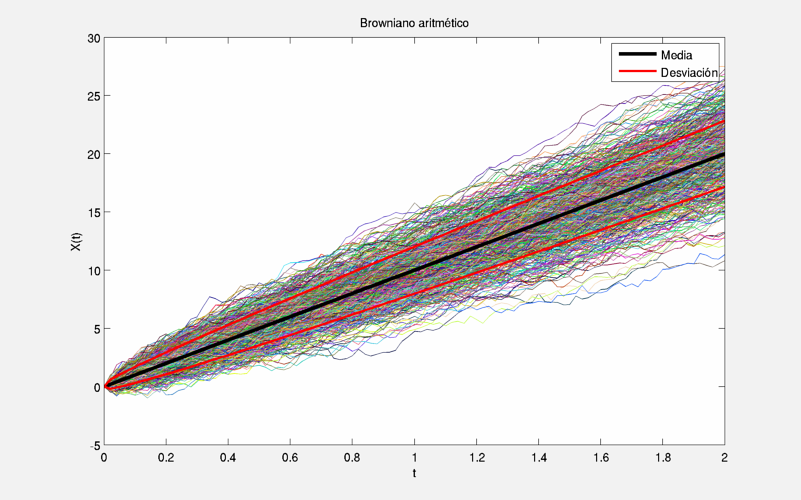
\includegraphics[scale=0.5,
      keepaspectratio]{./figures/ABM.png}
   \end{center}
   \caption{Browniano aritm\'etico}
\end{figure}

\textit{\textbf{NOTA}: todas las gr\'aficas representadas en este problema han
sido obtenidas con los par\'ametros por defecto que se especifican en los casos
de uso de cada uno de los programas suministrados en los anexos.}

\subsection{Diagrama de autocovarianzas}

Por la definici\'on de autocovarianza:

\begin{equation*}
   \mathrm{C}_{SS}(t,s) = \mathrm{E}[(S(t)-\mathrm{E}[S(t)])(S(s)-\mathrm{E}[S(s)])]
\end{equation*}

donde si $t = s$ la autocovarianza es la varianza, que ya conocemos a priori por los
resultados de la secci\'on anterior y servir\'a para comprobar si los resultados
tienen (algo) de sentido. Para ello comprobaremos que el segundo valor del
vector de autocovarianzas es $\sigma^2dT$.\\

Adem\'as de la observaci\'on anterior, sabemos la autocovarianza del ABM:

\begin{equation*}
   \tag{Autocovarianza}
   \mathrm{C}_{SS}(t,s) = \sigma^2 min(t,s)
\end{equation*}

luego, si $s$ es un intervalo en el que $t$ est\'a contenido, la autocovarianza
se saturar\'a cuando $s$ sobrepase a $t$. Por ejemplo,
la discretizaci\'on de la simulaci\'on para $n_1=30$ se corresponder\'ia con $t$ y
$s$ estar\'ia relacionado con la discretizaciones en un intervalo de $n_2 \in [1,
50]$.

\begin{figure}[htb]
   \begin{center}
      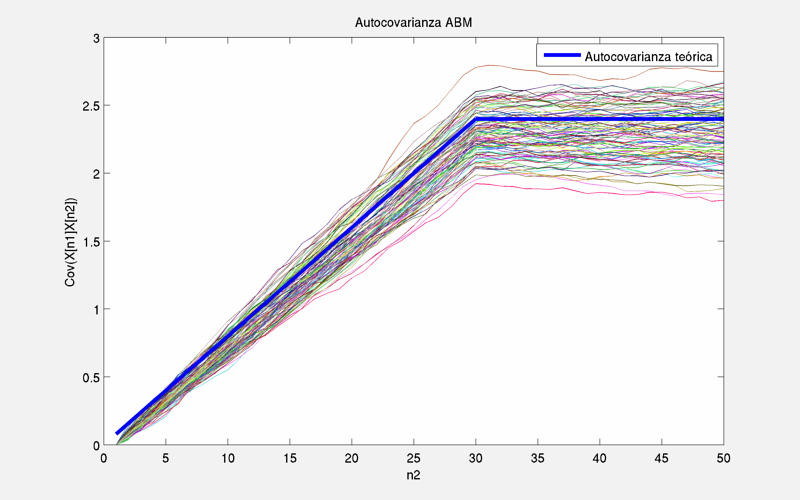
\includegraphics[scale=0.5,
      keepaspectratio]{./figures/autocovABM.png}
   \end{center}
   \caption{Autocovarianza para un ABM}
\end{figure}

Observamos la saturaci\'on de la autocovarianza en la simulaci\'on, tal y como
esper\'abamos.

\subsection{C\'odigo empleado}

Se han codificado tres archivos en Matlab:
\begin{itemize}
   \item \textbf{simBM.m}\\
      Funci\'on que calcula el browniano arim\'etico.
   \item \textbf{autocovBM.m}\\
      Funci\'on que calcula una matriz de autocovarianzas para un intervalo de
      tiempo dado sobre una referencia temporal.
   \item \textbf{plotautocovBM.m}\\
      Peque\~no programa para dibujar de una manera m\'as clara la
      autocovarancia calculada por medio de las simulaciones y la comparaci\'on
      con la te\'orica.
\end{itemize}

\newpage
\mbox{}

\pagebreak
\section{Valoraci\'on de productos derivados}

\subsection{Valoraci\'on de una call europea por cuadratura}

Para este problema procedemos id\'enticamente a como lo realizamos para el
problema 1: identificamos la funci\'on a integrar y realizamos una integraci\'on
por Lobatto.

Antes de obtener el precio, que es algo inmediato, analizamos de un
modo un tanto grosero la \textit{call} europea con los par\'ametros dados para
su simulaci\'on.

Primeramente observamos el precio del ejercicio a d\'ia de hoy que es:

\begin{equation*}
   K_{hoy} = e^{-rT}K = 84.7588
\end{equation*}

Luego comparamos con el precio a d\'ia de hoy del m\'aximo, valor
medio y m\'inimo de la evoluci\'on del subyacente por Black-Scholes:

\begin{center}
\begin{tabular}{|p{2.5cm}|p{3.5cm}|}
\hline
\multicolumn{2}{|c|}{\textbf{Valor del subyacente a d\'ia de hoy}}\\
\hline
\hline
\textbf{M\'aximo} & 150.0329\\
\hline
\textbf{Medio}    & 114.5944\\
\hline
\textbf{M\'inimo} & 85.2144\\
\hline
\end{tabular}
\end{center}

Es decir, vamos a pagar menos que el valor m\'inimo estimado, todo ello referido
a d\'ia de hoy. Podemos pensar que va a ser una operaci\'on
beneficiosa. Por \'ultimo, ojeamos un histograma del subyacente referido al presente. Para su
elaboraci\'on se tomaron $10^6$ muestras de una distribuci\'on $\mathcal{N}(0,1)$:

\begin{figure}[htb]
   \begin{center}
      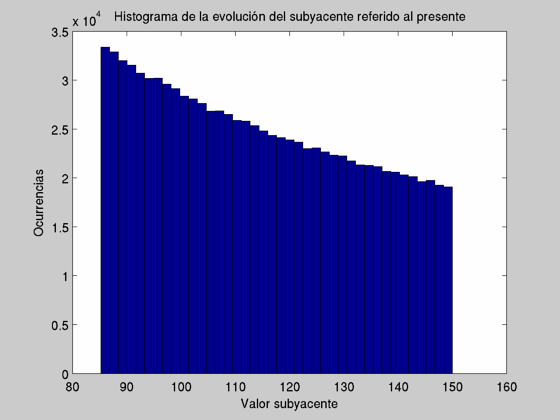
\includegraphics[scale=0.5,
      keepaspectratio]{./figures/histCallEUquad.png}
   \end{center}
   \caption{Evoluci\'on del subyacente referido al presente}
\end{figure}

Por \'ultimo, computamos el precio resultando 15,2187. La operaci\'on ser\'a
beneficiosa.

\subsection{Valoraci\'on de una call europea por simulaci\'on}

En primer lugar, enunciamos el \textbf{browniano geom\'etrico}, GBM:

\begin{equation*}
   \tag{\textbf{GBM}}
   \frac{dS_t}{S_t} = \mu dt + \sigma dW_t
\end{equation*}

cuya media y varianza son:

\begin{equation*}
   \tag{Media}
   \mathrm{E}[S(t)] = S_0 e^{(rt + \frac{\sigma ^2}{2}t)}
\end{equation*}

\begin{equation*}
   \tag{Varianza}
   \mathrm{E}[(S(t) - \mathrm{E}[S(t)])^2] = S_0^2 e^{(2rt +\sigma ^2t)}
   (e^{\sigma ^2} - 1)
\end{equation*}

Tanto para la \textit{call} europea como para la asi\'atica, evaluaremos con los siguientes
par\'ametros:

\begin{center}
\begin{tabular}{|p{3.5cm}|p{3.5cm}|}
\hline
\multicolumn{2}{|c|}{\textbf{Par\'ametros simulaci\'on}}\\
\hline
\hline
\textbf{Par\'ametro} & \textbf{Valor}\\
\hline
\hline
\textbf{M}      & 1000\\
\hline
\textbf{S0}     & 100\\
\hline
\textbf{K}      & 90\\
\hline
\textbf{r}      & 0.03\\
\hline
\textbf{T}      & 2\\
\hline
\textbf{$\sigma$} & 0.4\\
\hline
\end{tabular}
\end{center}

Para ejecutar la simulaci\'on hay que llamar a la funci\'on
\hyperref[precioCallEUMC]{\textit{precioCallEUMC.m}}. \'Este llama a la
funci\'on de pago, \hyperref[pagoCallEU]{\textit{pagoCallEU.m}}, tras la
construcci\'on del GBM en \hyperref[simGBM]{\textit{simGBM.m}}. De esta manera
obtenemos un browniano geom\'etrico como el siguiente que es consistente con
la teor\'ia sobre el GBM.

\begin{figure}[!htb]
   \begin{center}
      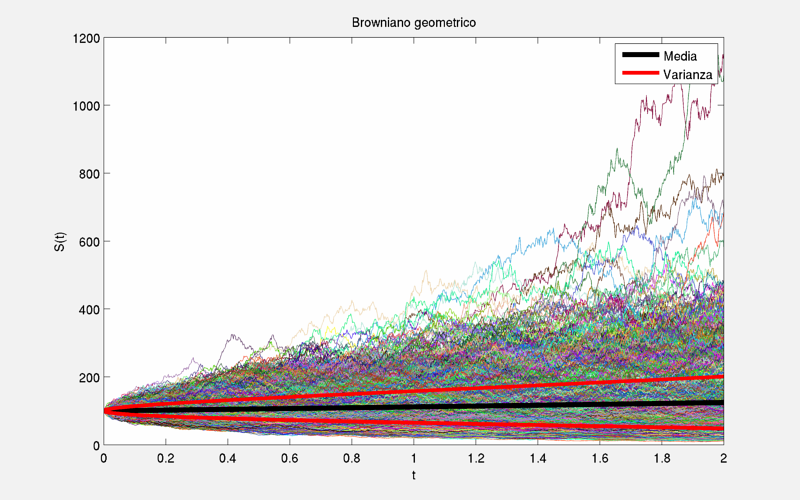
\includegraphics[scale=0.5,
      keepaspectratio]{./figures/GBM.png}
   \end{center}
   \caption{Browniano geom\'etrico}
\end{figure}


\subsubsection{Resultados}

Obtenemos los siguientes valores:

\begin{center}
\begin{tabular}{|p{3.5cm}|p{3.5cm}|}
\hline
\multicolumn{2}{|c|}{\textbf{Resultados}}\\
\hline
\hline
\textbf{Precio}     & 28.0038\\
\hline
\textbf{Error}      & 0.5025\\
\hline
\end{tabular}
\end{center}

que cambiar\'an ligeramente seg\'un realicemos simulaciones.

\pagebreak
\subsection{Valoraci\'on de una call asi\'atica de media aritm\'etica por simulaci\'on}

Los programas empleados guardan la misma estructura que en el caso anterior.
\hyperref[precioCallAsiaticaMC]{\textit{precioCallAsiaticaMC.m}} es el programa principal que
llama a la funci\'on de pago, \hyperref[pagoCallAsiatica]{\textit{pagoCallAsiatica.m}}, tras la
construcci\'on del GBM en \hyperref[simGBM]{\textit{simGBM.m}}.

\subsubsection{Resultados}

Tras ejecutar una simulaci\'on obtenemos:

\begin{center}
\begin{tabular}{|p{3.5cm}|p{3.5cm}|}
\hline
\multicolumn{2}{|c|}{\textbf{Resultados}}\\
\hline
\hline
\textbf{Precio}     & 29.0686\\
\hline
\textbf{Error}      & 0.5080\\
\hline
\end{tabular}
\end{center}

Es decir, la operaci\'on ser\'a beneficiosa en ambos casos.

\pagebreak

\newpage
\mbox{}

\pagebreak

\appendix
  \section{Problema 1}
    \subsection{centralMomentGaussian.m}

    \lstinputlisting[caption={centralMomentGaussian.m},
    label={centralMomentQuad}]{../matlab/exercise1/centralMomentGaussian.m}
    \subsection{quadfunction.m}
    \lstinputlisting[caption={quadfunction.m}, label={quadfunc}]{../matlab/exercise1/quadfunction.m}

  \pagebreak
  \section{Problema 2}
    \subsection{simBM.m}
    \lstinputlisting[caption={simBM.m},
    label={simBM}]{../matlab/exercise2/simBM.m}
    \subsection{autocovBM.m}
    \lstinputlisting[caption={simBM.m},
    label={autocovBM}]{../matlab/exercise2/autocovBM.m}
    \subsection{plotautocovBM.m}
    \lstinputlisting[caption={simBM.m},
    label={plotautocovBM}]{../matlab/exercise2/plotautocovBM.m}

  \pagebreak

  \section{Problema 3}
    \subsection{simGBM.m}
    \lstinputlisting[caption={simGBM.m},
    label={simGBM}]{../matlab/exercise3/simGBM.m}
    \pagebreak
    \subsection{pagoCallEU.m}
    \lstinputlisting[caption={pagoCallEU.m},
    label={pagoCallEU}]{../matlab/exercise3/pagoCallEU.m}
    \subsection{precioCallEU.m}
    \lstinputlisting[caption={precioCallEU.m},
    label={precioCallEU}]{../matlab/exercise3/precioCallEU.m}
     \subsection{precioCallEUMC.m}
     \lstinputlisting[caption={precioCallEUMC.m},
     label={precioCallEUMC}]{../matlab/exercise3/precioCallEUMC.m}
     \subsection{pagoCallAsiatica.m}
     \lstinputlisting[caption={pagoCallAsiatica.m},
     label={pagoCallAsiatica}]{../matlab/exercise3/pagoCallAsiatica.m}
     \subsection{precioCallAsiaticaMC.m}
     \lstinputlisting[caption={precioCallAsiaticaMC.m},
     label={precioCallAsiaticaMC}]{../matlab/exercise3/precioCallAsiaticaMC.m}

\end{document}
